\section{Methodology}
\label{section:methodology}

In this section, we present the architectural design of \textbf{Pyramid-ResMLP} and detail the mathematical formulation of our structural re-parameterization technique, \textbf{RepTokenMix}.

\subsection{Macro-architecture overview}
\label{subsection:macro_architecture}
Figure~\ref{fig:pyramid_resmlp_arch} illustrates the macro-architecture of Pyramid-ResMLP and contrasts it with the baseline Pyramid-ResMLP Pure. Given an input RGB image $X \in \mathbb{R}^{B \times 3 \times H \times W}$ (where $H = W = 64$ for Tiny-ImageNet-200), the network processes features through three hierarchical stages followed by a global pooling classifier.

\begin{figure}[htbp]
    \centering
    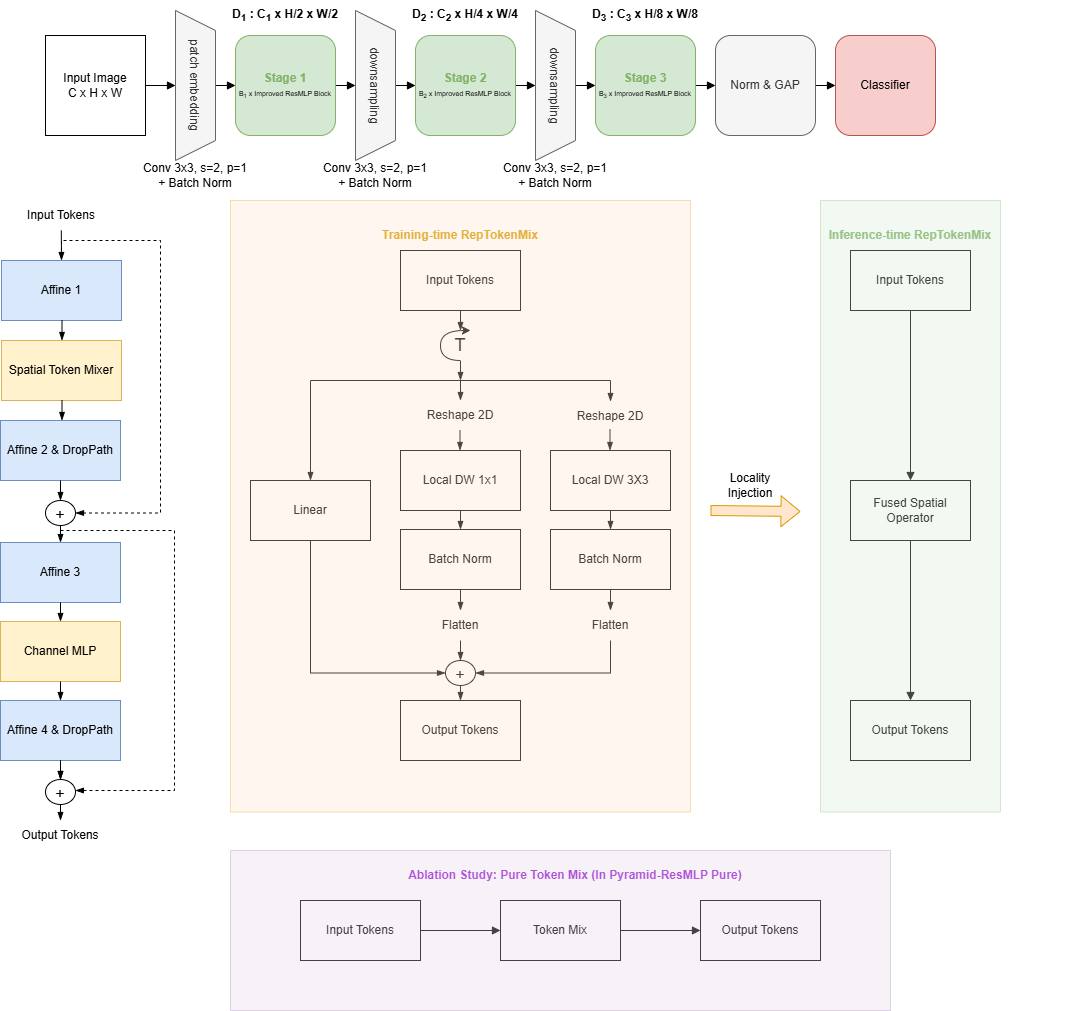
\includegraphics[width=0.98\linewidth]{figures/pyramid_resmlp_and_pure_arch.png}
    \caption{Macro-architecture comparison between Pyramid-ResMLP (left) and Pyramid-ResMLP Pure (right). Both models share an identical 3-stage pyramid layout with overlapping convolutional patch embeddings. Pyramid-ResMLP incorporates RepTokenMix with structural re-parameterization during training, collapsing into an efficient single linear layer at deployment.}
    \label{fig:pyramid_resmlp_arch}
\end{figure}

The structural specifications across all stages are summarized in Table~\ref{tab:arch_specs}.

\begin{table}[htbp]
\centering
\small
\begin{tabular}{lcccc}
\toprule
\textbf{Stage / Layer} & \textbf{Output Resolution} & \textbf{Tokens ($N$)} & \textbf{Channels ($C$)} & \textbf{Blocks ($B$)} \\
\midrule
Overlapping stem & $16 \times 16$ & 256 & 128 & -- \\
Stage 1 & $16 \times 16$ & 256 & 128 & 2 \\
Patch downsample 1 & $8 \times 8$ & 64 & 256 & -- \\
Stage 2 & $8 \times 8$ & 64 & 256 & 2 \\
Patch downsample 2 & $4 \times 4$ & 16 & 512 & -- \\
Stage 3 & $4 \times 4$ & 16 & 512 & 6 \\
Classifier head & $1 \times 1$ & 1 & 200 & -- \\
\bottomrule
\end{tabular}
\caption{Detailed architectural specifications of Pyramid-ResMLP for $64 \times 64$ input resolution.}
\label{tab:arch_specs}
\end{table}

\subsection{Overlapping convolutional stem}
\label{subsection:overlapping_stem}
Conventional vision MLPs extract non-overlapping patches (e.g., $4 \times 4$ linear projection with stride 4). This disjoint partitioning creates harsh boundary artifacts between adjacent patches because neighboring pixels situated across patch boundaries cannot interact in shallow layers.

To eliminate these boundary discontinuities, we design a two-layer overlapping convolutional stem:
\begin{enumerate}
    \item \textbf{Layer 1:} Conv2d with kernel size $7 \times 7$, stride 2, padding 3, mapping 3 input channels to 64 intermediate channels, followed by BatchNorm and GELU activation.
    \item \textbf{Layer 2:} Conv2d with kernel size $3 \times 3$, stride 2, padding 1, mapping 64 intermediate channels to $C_1 = 128$ stage-1 channels, followed by BatchNorm.
\end{enumerate}
This yields an initial downsampling factor of $4\times$, transforming the $64 \times 64 \times 3$ image into a spatial token grid of $16 \times 16$ ($N_1 = 256$) with channel dimension $C_1 = 128$. Because the kernels overlap across receptive fields, adjacent tokens share contextual pixels, establishing spatial continuity from the outset.

\subsection{Pyramid stages and downsampling layers}
\label{subsection:pyramid_stages}
Between consecutive stages, we insert patch downsampling layers. Each downsampling layer applies a strided $2 \times 2$ convolution with stride 2 and padding 0, followed by Layer Normalization:
\begin{equation}
    X_{s+1} = \text{LayerNorm}\Big(\text{Conv2D}_{2\times 2, \text{stride}=2}(X_s)\Big)
\end{equation}
This halving of the spatial dimensions ($16 \to 8 \to 4$) and doubling of the channel dimensions ($128 \to 256 \to 512$) accomplishes two critical objectives:
\begin{itemize}
    \item \textbf{Computational efficiency:} In the deepest stage (Stage 3, containing 6 blocks), the token count is reduced to only $N_3 = 16$. The spatial token-mixing matrix size is only $16 \times 16 = 256$ elements per channel, drastically lowering parameter and FLOP requirements compared to columnar architectures that retain 256 tokens at every depth.
    \item \textbf{Semantic hierarchy:} Shallow stages focus on dense spatial configurations, while deep stages process condensed semantic abstractions across 512 channels.
\end{itemize}

\subsection{Residual MLP block structure}
\label{subsection:block_structure}
Each residual block within stage $s$ consists of two residual sub-blocks: Token-Mixing and Channel-Mixing. Following the ResMLP formulation~\cite{touvron2021resmlp}, we stabilize training using learnable affine scale and bias vectors ($\text{Affine}(\cdot)$) and DropPath (stochastic depth)~\cite{huang2016deep}:
\begin{align}
    X' &= X + \text{DropPath}\Big(\text{Affine}_1\big(\text{TokenMix}(\text{Affine}_{\text{norm}1}(X))\big)\Big) \\
    Y &= X' + \text{DropPath}\Big(\text{Affine}_2\big(\text{ChannelMLP}(\text{Affine}_{\text{norm}2}(X'))\big)\Big)
\end{align}
The Channel-Mixing MLP applies an expansion ratio of $r = 4$ across the channel dimension:
\begin{equation}
    \text{ChannelMLP}(Z) = W_2 \cdot \text{GELU}(W_1 Z + b_1) + b_2, \quad W_1 \in \mathbb{R}^{4C \times C}, \; W_2 \in \mathbb{R}^{C \times 4C}
\end{equation}

\subsection{RepTokenMix and structural re-parameterization}
\label{subsection:reptokenmix}

\subsubsection{Training-time multi-branch formulation}
In standard ResMLP, the token-mixing operation is a pure global linear projection:
\begin{equation}
    \text{TokenMix}_{\text{pure}}(X) = W_{\text{fc}} X + b_{\text{fc}}, \quad W_{\text{fc}} \in \mathbb{R}^{N \times N}
\end{equation}
While $W_{\text{fc}}$ can theoretically learn any pairwise relationship between tokens, it lacks translation equivariance and locality.

In \textbf{RepTokenMix}, we augment this global linear projection with parallel local depthwise convolutional branches during training. For an input tensor $X \in \mathbb{R}^{B \times N \times C}$, we reshape it into a 2D spatial feature map $X_{2\text{D}} \in \mathbb{R}^{B \times C \times H_s \times W_s}$ (where $N = H_s \times W_s$). The training forward pass is defined as:
\begin{equation}
    \label{eq:reptoken_train}
    Y = W_{\text{fc}} X + \sum_{k \in \mathcal{K}} \text{flatten}\Big(\text{BN}_k\big(\text{DWConv}_k(X_{2\text{D}})\big)\Big) + b_{\text{fc}}
\end{equation}
where $\mathcal{K} = \{1, 3\}$ represents kernel sizes of $1 \times 1$ and $3 \times 3$ respectively. Each depthwise branch applies a grouped 2D convolution with groups equal to $C$, followed by Batch Normalization. The $3 \times 3$ branch provides immediate local inductive bias from adjacent tokens, while the $1 \times 1$ branch acts as a channel-wise identity shortcut.

\subsubsection{Inference-time fusion via impulse response}
Although multi-branch training accelerates convergence and boosts accuracy, evaluating multiple depthwise convolutions and batch normalizations at test time degrades GPU memory bandwidth and increases latency.

Because depthwise convolution, batch normalization, and fully-connected projections are all \textbf{linear transformations}, their sum can be analytically merged into a single equivalent weight matrix $W_{\text{deploy}} \in \mathbb{R}^{C \times N \times N}$ and bias vector $b_{\text{deploy}} \in \mathbb{R}^{C \times N}$.

First, we absorb the Batch Normalization parameters (running mean $\mu$, running variance $\sigma^2$, weight $\gamma$, and bias $\beta$) directly into the depthwise convolution kernel $K \in \mathbb{R}^{C \times 1 \times k \times k}$ and bias $b$:
\begin{equation}
    \widehat{K}_c = \frac{\gamma_c}{\sqrt{\sigma_c^2 + \epsilon}} K_c, \qquad \widehat{b}_c = \beta_c - \frac{\gamma_c \mu_c}{\sqrt{\sigma_c^2 + \epsilon}}
\end{equation}

Second, to convert the 2D depthwise convolution $\widehat{K}_c$ into an equivalent $N \times N$ spatial matrix $W_{\text{conv}}^{(c)}$, we exploit the \textbf{impulse response property}. We construct a Dirac delta identity tensor $I \in \mathbb{R}^{C \times N \times H_s \times W_s}$ such that for each spatial token $j \in \{1, \dots, N\}$:
\begin{equation}
    I_{c, j, y, x} = 
    \begin{cases} 
        1 & \text{if } (y, x) = \text{coord}(j) \\
        0 & \text{otherwise}
    \end{cases}
\end{equation}
By convolving $I$ with the folded kernel $\widehat{K}$, the output response at token location $i$ directly yields the coefficient connecting token $j$ to token $i$:
\begin{equation}
    W_{\text{conv}}^{(c)}[i, j] = \Big(\widehat{K}_c * I_{c, j}\Big)\big[\text{coord}(i)\big]
\end{equation}

Finally, because the global linear layer $W_{\text{fc}} \in \mathbb{R}^{N \times N}$ shares weights across all channels, it is broadcast along the channel dimension. The unified deployment parameters are computed as:
\begin{align}
    W_{\text{deploy}}^{(c)} &= W_{\text{fc}} + \sum_{k \in \mathcal{K}} W_{\text{conv}, k}^{(c)}, \quad \forall c \in \{1, \dots, C\} \\
    b_{\text{deploy}}^{(c)} &= b_{\text{fc}} + \sum_{k \in \mathcal{K}} \widehat{b}_k^{(c)}
\end{align}

At test time, the entire RepTokenMix layer executes as a single batched matrix multiplication:
\begin{equation}
    Y_{\text{deploy}}[:, i, c] = \sum_{j=1}^N W_{\text{deploy}}^{(c)}[i, j] X[:, j, c] + b_{\text{deploy}}^{(c)}[i]
\end{equation}
This deployment operation requires \textbf{zero depthwise convolutions, zero batch normalization layers, and zero branching overhead}, guaranteeing strict zero-overhead inference.
